\begin{definition}{Recherche Informée}{informedsearch}

    La recherche \textbf{informée} est une stratégie de recherche qui utilise \textbf{des informations} sur l'état de l'environnement afin de le \textbf{guider} pour trouver une solution.
    Elle explore l'espace de recherche de manière \textbf{intelligente} gràce à des \textbf{heuristiques}. 
    Ces heuristiques permettent de \textbf{quantifier} la \textbf{qualité} d'un état et donc 
    de guider la recherche vers les états les plus prometteurs.
\end{definition}

\begin{remark}\leavevmode
    La performance de ces algorithmes dépendent de la qualité de l'heuristique utilisée.
\end{remark}

\begin{definition}{Heuristique}{heuristic}
    Une heuristique est une fonction qui permet d'estimer à quel point un état est \textbf{proche}
    de l'état final. Elles sont designées pour des problèmes spécifiques.
\end{definition}

\begin{examples}\leavevmode
    \begin{enumerate}
        \item \textbf{Distance Euclidéenne}: la distance entre deux points 
            en ligne droite 
        \item \textbf{Distance de Manhattan}: la distance entre deux points 
            en ligne droite mais en ne pouvant se déplacer que sur les axes 
            (pas en diagonale) 
    \end{enumerate}
\end{examples}


\subsection{Greedy Best-First Search} % (fold)
\label{sub:greedy_best_first_search}

\begin{definition}{Greedy Best-First Search}{greedybestfirstsearch}
    La recherche gloutonne (\textbf{Greedy Best-First Search}) est une stratégie de recherche qui explore l'arbre en choisissant le noeud qui semble le plus prometteur.
    \begin{itemize}
        \item \textbf{Frontière}: une file de priorité
        \item \textbf{Stratégie}: on choisit le noeud ayant la meilleure heuristique de la frontière (en  fonction de la stratégie)
    \end{itemize} 
\end{definition}

\begin{figure}[H]
  \centering
  \scalebox{0.65}{
  \begin{minipage}[b]{0.30\textwidth}
    \centering
    \begin{tabular}[c]{|ll|ll|}
        \hline
        % \multicolumn{1}{c|}{\textbf{}} & 
        % \multicolumn{1}{c}{\textbf{}} \\
        % \hline
        \textbf{Arad} & 366 & \textbf{Mehadia} & 241 \\ 
        \textbf{Bucharest} & 0 & \textbf{Neamt} & 234 \\ 
        \textbf{Craiova} & 160 & \textbf{Oradea} & 380 \\ 
        \textbf{Dobreta} & 242 & \textbf{Pitesti} & 100 \\ 
        \textbf{Eforie} & 161 & \textbf{Rimnicu Vilcea} & 193 \\ 
        \textbf{Fagaras} & 176 & \textbf{Sibiu} & 253 \\ 
        \textbf{Giurgiu} & 77 & \textbf{Timisoara} & 329 \\ 
        \textbf{Hirsova} & 151 & \textbf{Urziceni} & 80 \\ 
        \textbf{Iasi} & 226 & \textbf{Vaslui} & 199 \\ 
        \textbf{Lugoj} & 244 & \textbf{Zerind} & 374 \\ 
        \hline
    \end{tabular}

    \caption{Tableau de valeure d'heuristique}
    \label{tab:heuristics}
  \end{minipage}
   }
  \hfill
  \scalebox{0.7}{
  \begin{minipage}{0.70\textwidth}
    \centering
    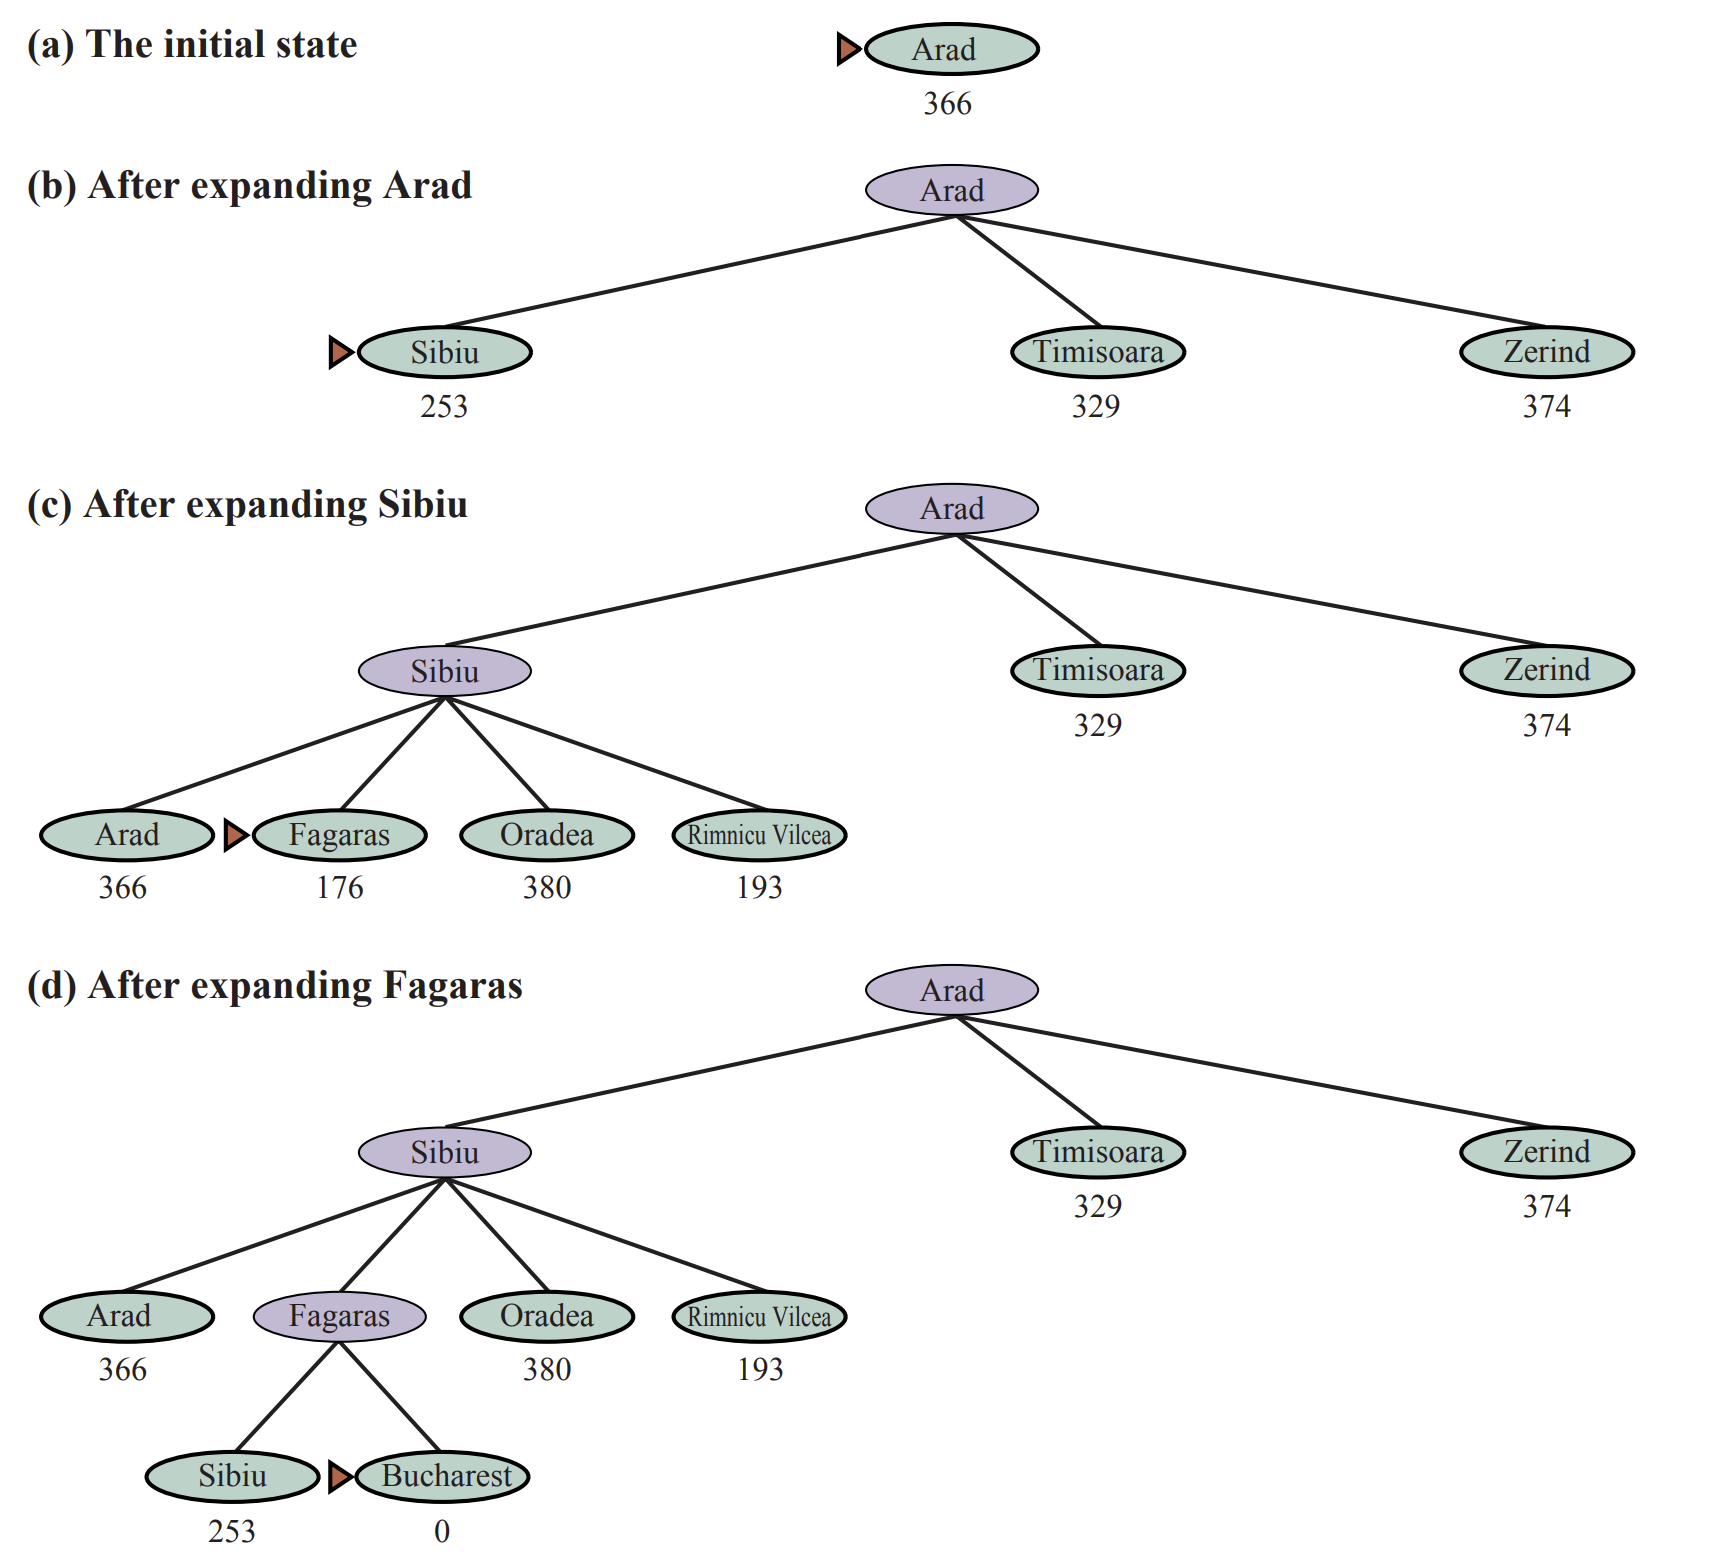
\includegraphics[width=\textwidth]{./pictures/greedy.png}
    \caption{Exécution de l'algo greedy}
    \label{fig:greedy}
  \end{minipage}
    }
\end{figure}


\begin{remarks}\leavevmode
    \begin{enumerate}
        \item \textbf{Complet}: Non, peut aller dans des profondeurs infinies
        \item \textbf{Optimal}: Non
        \item \textbf{Complexité en temps}: $O(b^m)$
        \item \textbf{Complexité en espace}: $O(b^m)$
        \item Il est en général meilleur que \textbf{DFS}
    \end{enumerate}
\end{remarks}

% subsection Greedy Best-First Search (end)

\subsection{A*} % (fold)
\label{sub:a_}

\begin{definition}{A*}{astar}
    L'algorithme \textbf{A*} est une stratégie de recherche qui explore l'arbre en choisissant le noeud qui semble le plus prometteur.
    \begin{itemize}
        \item \textbf{Frontière}: une file de priorité
        \item \textbf{Stratégie}: on choisit le noeud ayant le plus petit coût de la frontière
    \end{itemize} 
    La fonction d'évaluation est la suivante: 
    \begin{math}
        f(n) = g(n) + h(n)
    \end{math} 
    où $g(n)$ est le coût pour atteindre le noeud $n$ depuis la racine et 
    $h(n)$ est le cout du noeud $n$ pour aller jusqu'au but (\textit{heuristique}).
\end{definition}

\begin{figure}[H]
    \begin{center}
        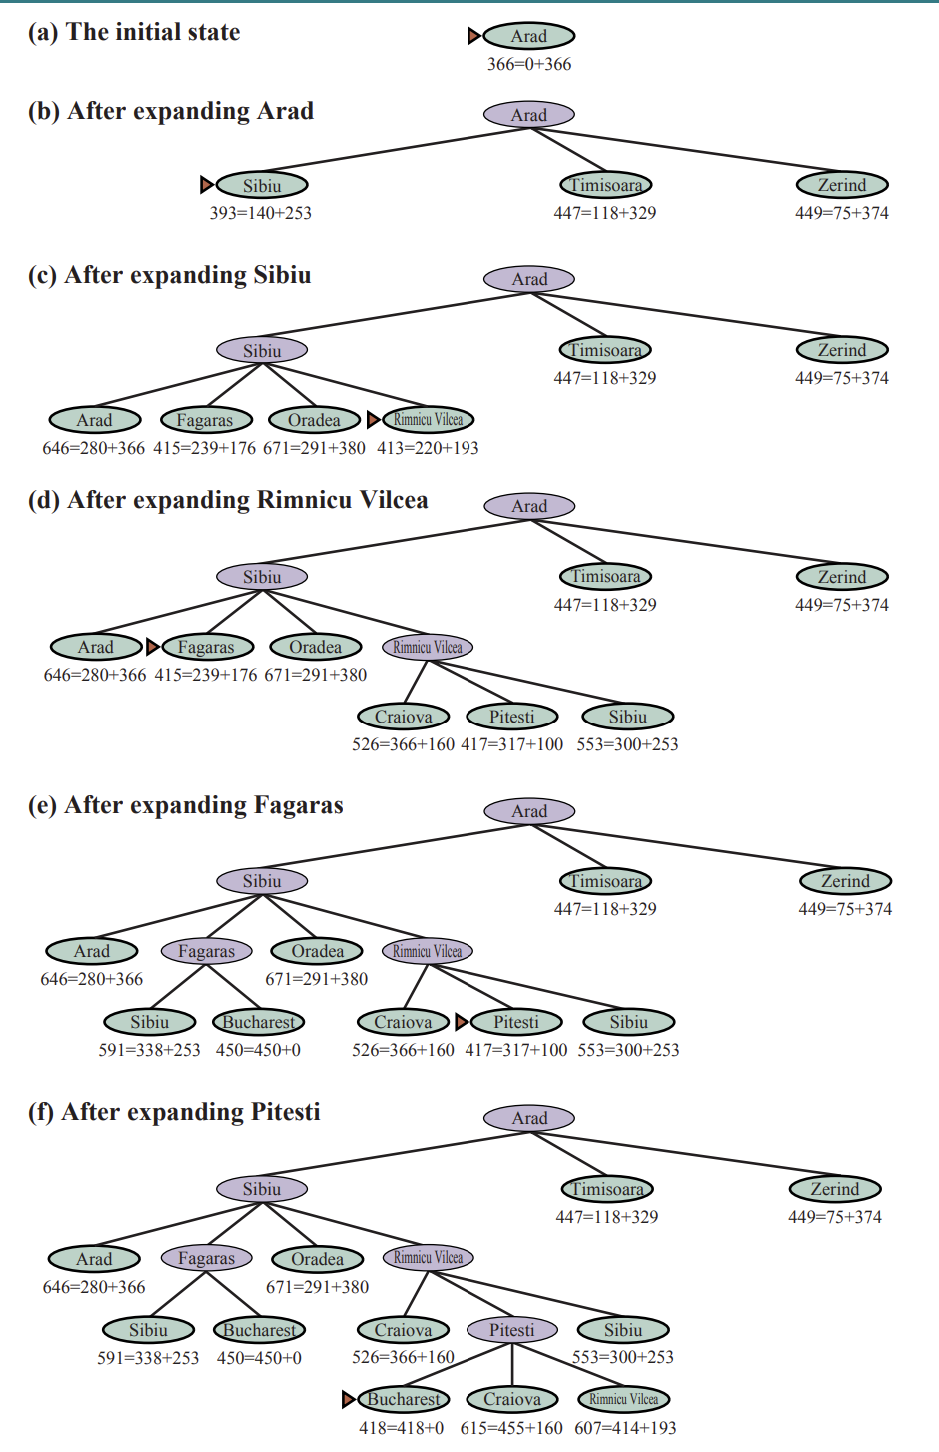
\includegraphics[width=0.5\textwidth]{./pictures/astar.png}
    \end{center}
    \caption{Exécution de l'algo A*}\label{fig:astar}
\end{figure}

\begin{remarks}\leavevmode
    \begin{enumerate}
        \item \textbf{Complet}: Oui
        \item \textbf{Optimal}: Oui si $h(n)$ est admissible
        \item \textbf{Complexité en temps}: $O(b^d)$
        \item \textbf{Complexité en espace}: $O(b^d)$
    \end{enumerate}
\end{remarks}
% subsection A* (end)

\subsection{Creer des Heuristiques admissibles} % (fold)
\label{sub:creer_des_heuristiques_admissibles}

\begin{definition}{Admissible}{admissible}
    Une heuristique est admissible si elle ne surestime jamais le coût pour atteindre l'état final. 
    \begin{math}
        h(n) \leq h^*(n) 
    \end{math} 
    où $h^*(n)$ est le coût réel pour atteindre l'état final. 
    C'est une fonction \textbf{optimiste}
\end{definition}

\begin{definition}{Cohérent}{consitent}
    Une \textbf{heuristique} est \textbf{cohérente} si, pour chaque noeud $n$ et un successeur $n'$ de $n$ généré par une action $a$,
    le coût estimé pour atteindre l'état final depuis $n$ est inférieur ou égal au coût de l'action $a$ plus le coût estimé pour atteindre l'état final depuis $n'$. 
    \begin{math}
        h(n) \leq c(n, a, n') + h(n') 
    \end{math} 
    où $c(n, a, n')$ est le coût de l'action $a$ pour aller de $n$ à $n'$. 
    Sinon, ça veut dire que l'heuristique surestime le coût pour atteindre l'état final.
\end{definition}

\begin{remark}\leavevmode
    Une heuristique cohérente est toujours admissible. 
\end{remark}

\begin{note}
    Lorsqu'on compare 2 heuristiques, on peut dire que l'heuristique $h_1$ est meilleure que $h_2$ si 
    \begin{math}
        h_1(n) \leq h_2(n) \forall n 
    \end{math}
\end{note}

Afin de créer une heuristique admissible, on peut utiliser les méthodes suivantes: 
\begin{itemize}
    \item \textbf{Relaxation}: on simplifie le problème en enlevant des contraintes
    \item \textbf{Décomposition}: on décompose le problème en sous-problèmes qui sont plus facile à résoudre
    \item \textbf{Combinaison}: on combine plusieurs heuristiques 
\end{itemize}

Il est aussi possible de stocker les valeures réelles dans une \textbf{base de donnée} 
et de les utiliser pour calculer l'heuristique (qui est dcp dans la bdd).
% subsection Creer des Heuristiques admissibles (end)

